% Created 2014-12-19 Fri 15:44
\documentclass[9pt,b5paper]{article}
\usepackage{graphicx}
\usepackage{xcolor}
\usepackage{xeCJK}
\setCJKmainfont{SimSun}
\usepackage{longtable}
\usepackage{float}
\usepackage{textcomp}
\usepackage{geometry}
\geometry{left=0cm,right=0cm,top=0cm,bottom=0cm}
\usepackage{multirow}
\usepackage{multicol}
\usepackage{listings}
\usepackage{algorithm}
\usepackage{algorithmic}
\usepackage{latexsym}
\usepackage{natbib}
\usepackage{fancyhdr}
\usepackage[xetex,colorlinks=true,CJKbookmarks=true,linkcolor=blue,urlcolor=blue,menucolor=blue]{hyperref}


\lstset{language=c++,numbers=left,numberstyle=\tiny,basicstyle=\ttfamily\small,tabsize=4,frame=none,escapeinside=``,extendedchars=false,keywordstyle=\color{blue!70},commentstyle=\color{red!55!green!55!blue!55!},rulesepcolor=\color{red!20!green!20!blue!20!}}
\author{Jenny Huang}
\date{\today}
\title{Android App Programming Directed Study \textasciitilde{} DrawingFun}
\hypersetup{
  pdfkeywords={},
  pdfsubject={},
  pdfcreator={Emacs 24.3.1 (Org mode 8.2.7c)}}
\begin{document}

\maketitle
%\tableofcontents


\section{Course Goal and General Review}
\label{sec-1}
\begin{itemize}
\item Taking this course, I wanted to help myself stay on schedule and learn some cutting-edge knowledge as a starting point.
\item I never had any "new" knowledge like "Android" learned before, this is the first time, and I enjoy it;
\item I enjoyed two modules the most: the color popup dialog and undo/redo functionalities. And in the middle, ListView helped a little bit as well;
\begin{itemize}
\item The color picker was not my original work, but for me at that time, it was very complicated and it forced me to understand all the Android framework for an App to function, the manifest, layout, value etc;
\item To implement a fully functional ListView together with the rest of the functionalities, I figured out my own way of creating a bridge SuperActivity class, which in terms of Java-programming, created a starting point of confidence that I can implement my ideas (any ideas) in Java as far as I \textbf{think} it through, clear. It is always the ideas that matter, instead of any implementation.
\item For undo/redo interface/implementation, I had thought to skip around by implementing Command Patterns, but now I am glad that Dr. Jeffery insisted us to apply interface/implementation. And I had been frustrated yet more than happy take my own effort to try, step by step, implement and see eventually it is working\textasciitilde{}! And during this process, I felt I began to be exposed to Java OOD, Android canvas, bitmap, drawing primitives, and I understood the theory behind them now, even only the parts that I implemented.
\end{itemize}
\end{itemize}

\section{Functionalities and User Interface}
\label{sec-2}
\subsection{Functionalities}
\label{sec-2-1}
\begin{itemize}
\item \textbf{New, Draw, Save, Erase:} These four functions were originally included in the starting point app already; I just modified "\textbf{Erase}" functionalities so that according to my drawing primitives, which will be included below, I can erase in different shapes, like smooth line, triangle, rectangle, sqare, circle etc.
\item \textbf{Color Picker:} Changed the app default 12-color choices into a color-picker square. This functionalities was difficult enough that even by connecting the necessary parts together and integrating them into my app, it took me hours and eventually I understood the whole process.
\item \textbf{Drawing Primitives:} Also referred to a website like I did on color-picker, but integrated into my app required my efforts on it, and it was inspiring.
\item \textbf{Undo/Redo:} Got google help and had starting point, but design the implementation method took me some while to get into it.
\item \textbf{Open:} A functionality that I tried and ended up helped in FloodFill for background bitmap;
\item \textbf{FloodFill:} Simply referred to websites, tried AsyncTask and Thread two methods, and applied the latter.
\end{itemize}
\subsection{Screenshots}
\label{sec-2-2}
\begin{itemize}
\item Color-picker
\end{itemize}
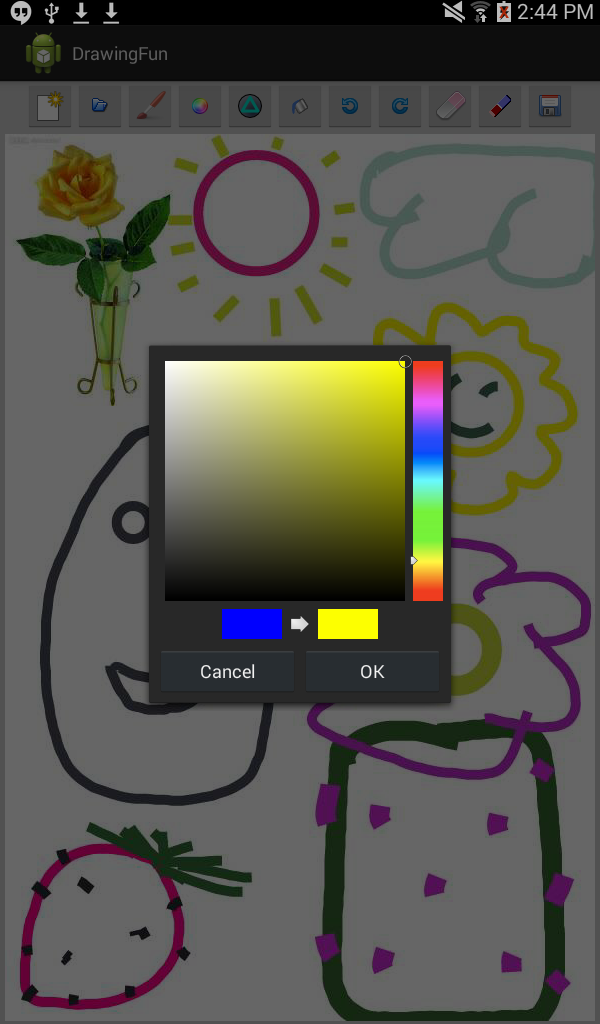
\includegraphics[width=.3\linewidth]{./Screenshot_2014-12-18-14-44-41.png}
\begin{itemize}
\item Drawing Primitives
\end{itemize}
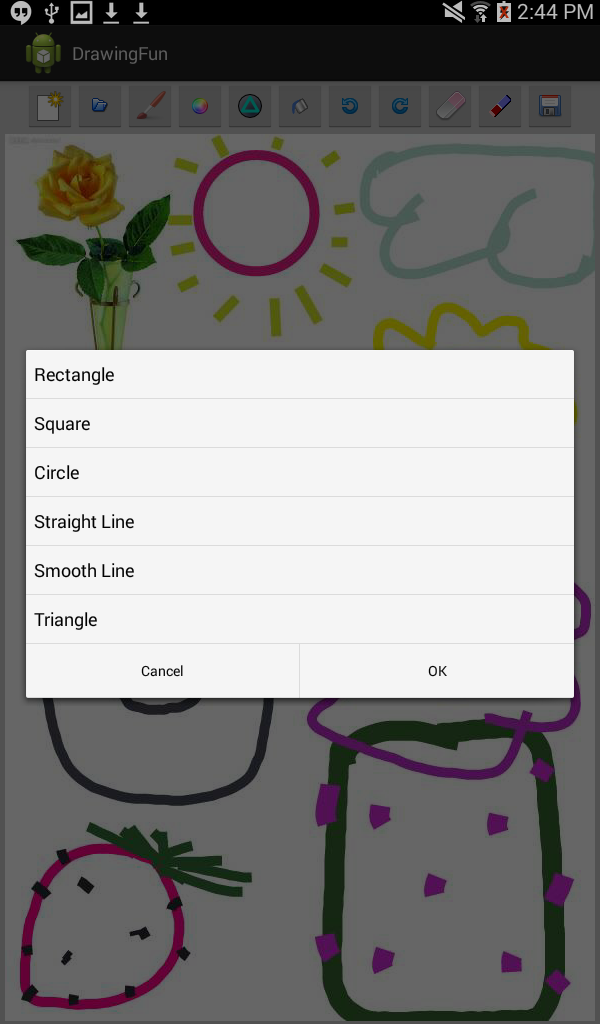
\includegraphics[width=.3\linewidth]{./Screenshot_2014-12-18-14-44-54.png}

\section{Implementation}
\label{sec-3}
\begin{itemize}
\item \textbf{Base app} was applied and it I didn't step into it for any code at that time;
\item \textbf{Color-picker} and \textbf{drawing primitives} are points of my interests. They were not my original work, but it required necessary understanding to integrate the function modules into one functional app. I took my challange and integrated ListView to work with my current app;
\item \textbf{Undo/Redo} worth the biggest challange for me. The starting point referred to a website seemed to be easy, but to apply this functionalities to all the drawing primitives, I got helped from the course instructor about interface and different implementation. I digested this interface/implementation concepts completely, and fully understood the primitives design, and designed and implemented the undo/redo functionalities. It worked pretty good, especially for triangle considering its drawing mechanism, except that I didn't think deep into how to make angles smoother than there are right now.
\end{itemize}

\section{Course Benefits}
\label{sec-4}
\begin{itemize}
\item The latter half semester of implementing DrawFun Paint project helped me realize that I can perform great in concentrated topics, which helps me focus.
\item It has been a challanging and interesting learning experience during this Android App Programming, and it successfully reached the target which I expected from this course. I learned the basic necessary knowledge to build my Android App and Java Programming background, and I practiced and cultivated the necessary and usefull skills to think logically, solve problems and debug my codes.
\item The course built knowledge, practiced skills, as well as built confidence in programming and problem-solving, and help cultivated my \textbf{I CAN DO} attitude towards projects.
\item After taking this course, I have a sufficient starting point to self-learn and practice Android App Programming. And now I am ready to prefer Java over c++ as my primary and first choice programming language, and I will try to conduct more practice on Java programming so I can be proficient on it in not far future.
\end{itemize}

\section{Reference}
\label{sec-5}
\begin{itemize}
\item Base App: \url{http://code.tutsplus.com/tutorials/android-sdk-create-a-drawing-app-interface-creation-mobile-19021}
\item Drawing Shapes with Finger: \url{http://gmariotti.blogspot.com/2014/01/drawing-shapes-with-fingers.html}
\item Load Image: \url{http://www.learn2crack.com/2014/06/android-load-image-from-internet.html}
\item Path() library: \url{http://grepcode.com/file/repository.grepcode.com/java/ext/com.google.android/android/2.3.1_r1/android/graphics/Path.java}
\item Mutable Bitmap: \url{http://stackoverflow.com/questions/13119582/android-immutable-bitmap-crash-error}
\item Undo/Redo Start: \url{http://stackoverflow.com/questions/11114625/android-canvas-redo-and-undo-operation}
\item FloodFill AsyncTask: \url{http://stackoverflow.com/questions/12669740/android-using-flood-fill-algorithm-getting-out-of-memory-exception}
\item FloodFill Thread: \url{http://stackoverflow.com/questions/8070401/android-flood-fill-algorithm}
\item I missed one reference. I remembered I refered to some website for color-picker, but I lost track for it. But to be clear, I did refer to the website, and it was NOT my original work.
\end{itemize}
% Emacs 24.3.1 (Org mode 8.2.7c)
\end{document}